\newpage
\appendix
%redefine figure and table counters
\renewcommand\thefigure{S\arabic{figure}}    
\setcounter{figure}{0} 
\renewcommand\thetable{S\arabic{table}}    
\setcounter{table}{0}

\section{Appendix: Sensitivity of the optimisation procedure to initial values}
\subsection{Approach}
\label{sec:appendix}
The sensitivity of parameter estimates for the cumulative model with constant variance (Eqn.~\ref{eq:candy_cm_count_form}) obtained using the direct likelihood optimisation with \verb+optim+ was assessed by simulation.
Simulations consisted of drawing a set of random initial values. To preserve the ordering of the cut-point parameters $\alpha_i$, their initial values $\alpha^{\circ}_i$ were assembled as the cumulative sum of six independent draws $$x_j \sim \mathrm{Uniform}(1,20), \qquad j = 1,\ldots, 6$$ i.e. $$\alpha^{\circ}_i = \sum_{j=1}^i x_j.$$ The initial value for $\beta$ was drawn as $$\beta^{\circ}\sim\mathrm{Uniform}(-1,1).$$

Optimisation proceeded using the likelihood outlined in Section~\ref{sec:const_var_cm} with a numerical threshold at the machine's precision to prevent the Poisson likelihood from approaching negative infinity. The optimisation routine used the BFGS method and parameter scaling value for $\beta$ of 0.01 relative to the cut-point parameters $\alpha_i$. This improved overall convergence rates but allowed convergence at an infinite likelihood, the likelihood was therefore evaluated one final time without thresholding at the converged parameter values and parameters were only retained when the unthresholded likelihood was finite. 
Parameters were further filtered to remove parameter sets where convergence was achieved at a finite likelihood, but with a substantially larger overall log-likelihood than the best model fit. Thresholds for this were determined empirically and set at 93 for the logit link and 100 for the cloglog model.

\subsection{Results}
The optimisation was reasonably robust for the logit link model. 73\% of simulations achieved convergence at a finite likelihood and of these over 99\% met the filtering threshold (Figure~\ref{fig:figS1}). Among the filtered parameter sets variability in the final estimates was very small (para\-meter-wise coefficients of variation were all smaller than 0.01\%) and there was no correlation between initial values and parameter estimates when taking into account that multiple comparisons were made (Table~\ref{tab:tabS2}). Convergence failed for initial values $\beta^{\circ}>0.7$, and convergence failures were likely, but not guaranteed for $\beta^{\circ}\approx 0$ (Figure~\ref{fig:figS2}).

The optimisation of the cloglog model was less stable. Only 47\% of simulations resulted in convergence, and of those 92\% met the filtering threshold (Figure~\ref{fig:figS1}). Variability in the filtered parameter estimates was larger than for the logit model, but still small in absolute terms (parameter-wise coefficients of variation were all below 0.01\%) and there was no correlation between initial values and parameter estimates (Table~\ref{tab:tabS2}). Convergence failed for many $0<\beta^{\circ}<0.2$, and always for $\beta^{\circ}>0.2$ (Figure~\ref{fig:figS3}). 


\begin{table}[bph]
  \small
    \centering
    \caption{Summary statistics of parameter sensitivities to starting values for the cumulative model with constant variance (Eqn.~\ref{eq:candy_cm_count_form}). The coefficients of variation (CV), correlation coefficients between initial and converged values $\rho^{\circ}$, and their corresponding p-values $P_\rho$ were calculated for the filtered parameter estimates only and adjusted for multiple comparisons using the Bonferroni correction.
    }
  
\begin{tabular}{cccccccc}
\toprule
Par. & Link & Sim. range & Conv. range & Filtered range & CV (\%) & $\rho^{o}$ & $P_\rho$\\
\midrule
a1 & logit & 1.3 - 20 & 1.3 - 20 & 1.3 - 20 & 0.692 & 0.101 & 0.115\\
a2 & logit & 3.1 - 37.8 & 3.1 - 37.6 & 3.1 - 37.6 & 0.677 & 0.138 & 0.031\\
a3 & logit & 5.4 - 54.1 & 5.4 - 54.1 & 5.4 - 54.1 & 0.627 & 0.123 & 0.055\\
a4 & logit & 13 - 69.9 & 15.9 - 69.9 & 15.9 - 69.9 & 0.558 & 0.079 & 0.220\\
a5 & logit & 22.9 - 85 & 22.9 - 85 & 22.9 - 85 & 0.548 & 0.006 & 0.929\\
a6 & logit & 31.6 - 100.7 & 32.7 - 100.7 & 32.7 - 100.7 & 0.601 & -0.010 & 0.873\\
b & logit & -1 - 1 & -1 - 0.8 & -1 - 0.8 & 0.570 & -0.106 & 0.097\\
\addlinespace
a1 & cloglog & 1.1 - 19.9 & 1.1 - 19.9 & 1.2 - 18.7 & 1.986 & 0.034 & 0.778\\
a2 & cloglog & 3.3 - 38.9 & 4 - 37.3 & 4 - 34.4 & 1.774 & -0.045 & 0.709\\
a3 & cloglog & 7.9 - 57 & 9.7 - 52.4 & 9.7 - 50.7 & 1.708 & -0.025 & 0.837\\
a4 & cloglog & 15 - 67 & 16.3 - 66.9 & 16.3 - 63.8 & 1.689 & -0.055 & 0.651\\
a5 & cloglog & 18.4 - 77.8 & 18.4 - 77.8 & 18.4 - 77.8 & 1.627 & 0.010 & 0.935\\
a6 & cloglog & 22.8 - 91.6 & 30.7 - 91.6 & 30.7 - 83.2 & 1.663 & 0.039 & 0.751\\
b & cloglog & -1 - 1 & -1 - 0.2 & -1 - 0.2 & 1.678 & -0.034 & 0.779\\
\bottomrule
\end{tabular}
  \label{tab:tabS2}
\end{table}


\begin{figure}[htbp]
  \centering
  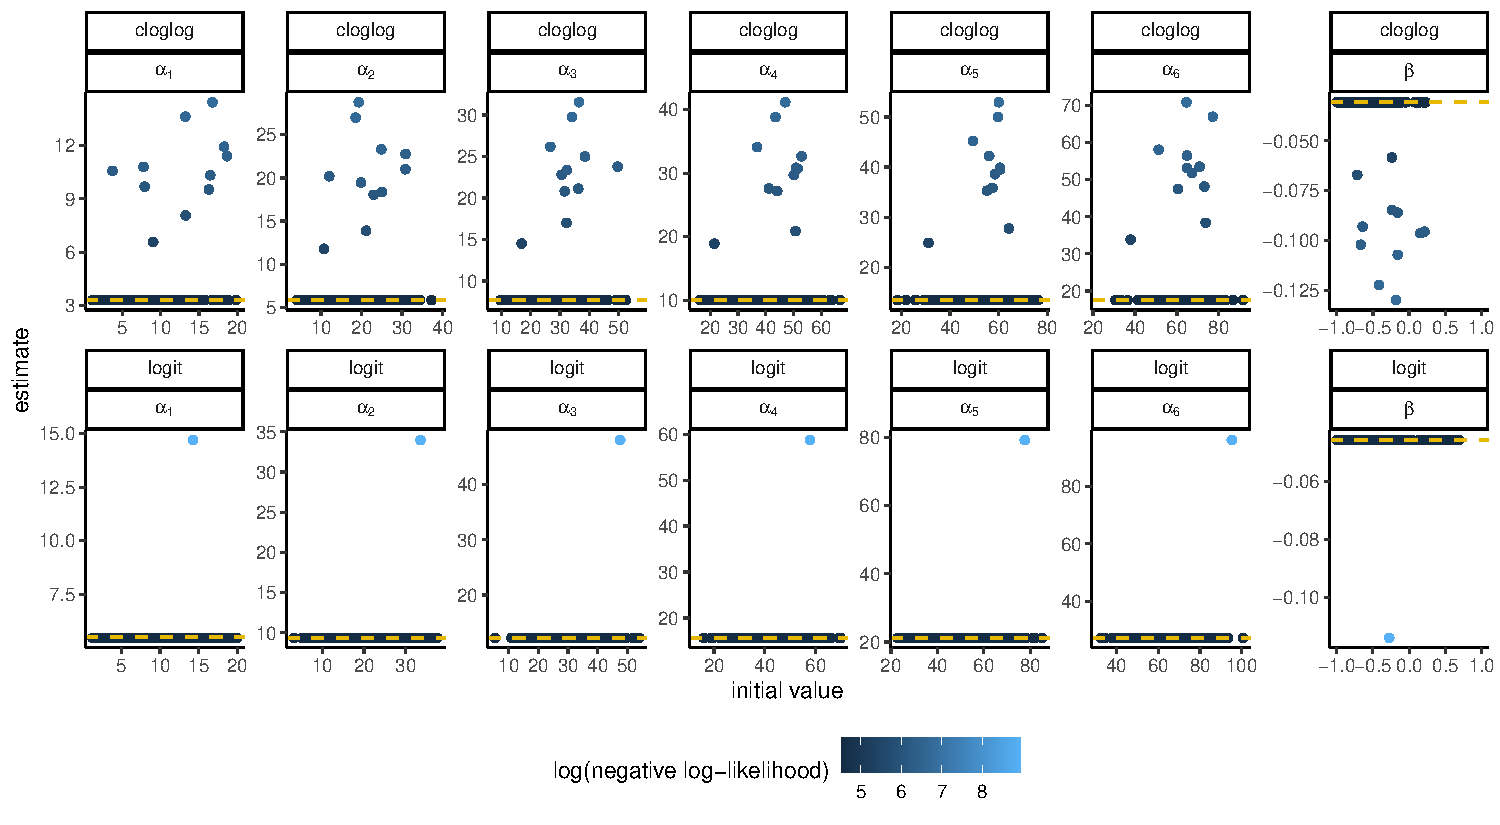
\includegraphics[width=\textwidth]{../figures/figS1_initial_value_sensitivity_unfiltered.pdf}
  \caption{Optimisation results for randomly drawn initial values for the cumulative model with constant variance. Parameter estimates are coloured by the log of the negative log-likelihood of the corresponding model fit. Yellow dashed lines correspond to parameter values reported in \citep{candy1991modeling}. The majority of initial values resulted in estimates close to the original publication for the logit model (bottom). Convergence to local optima far from the published parameters was more common in the cloglog link model (top).}
  \label{fig:figS1}
\end{figure} 

\begin{figure}[p]
  \centering
  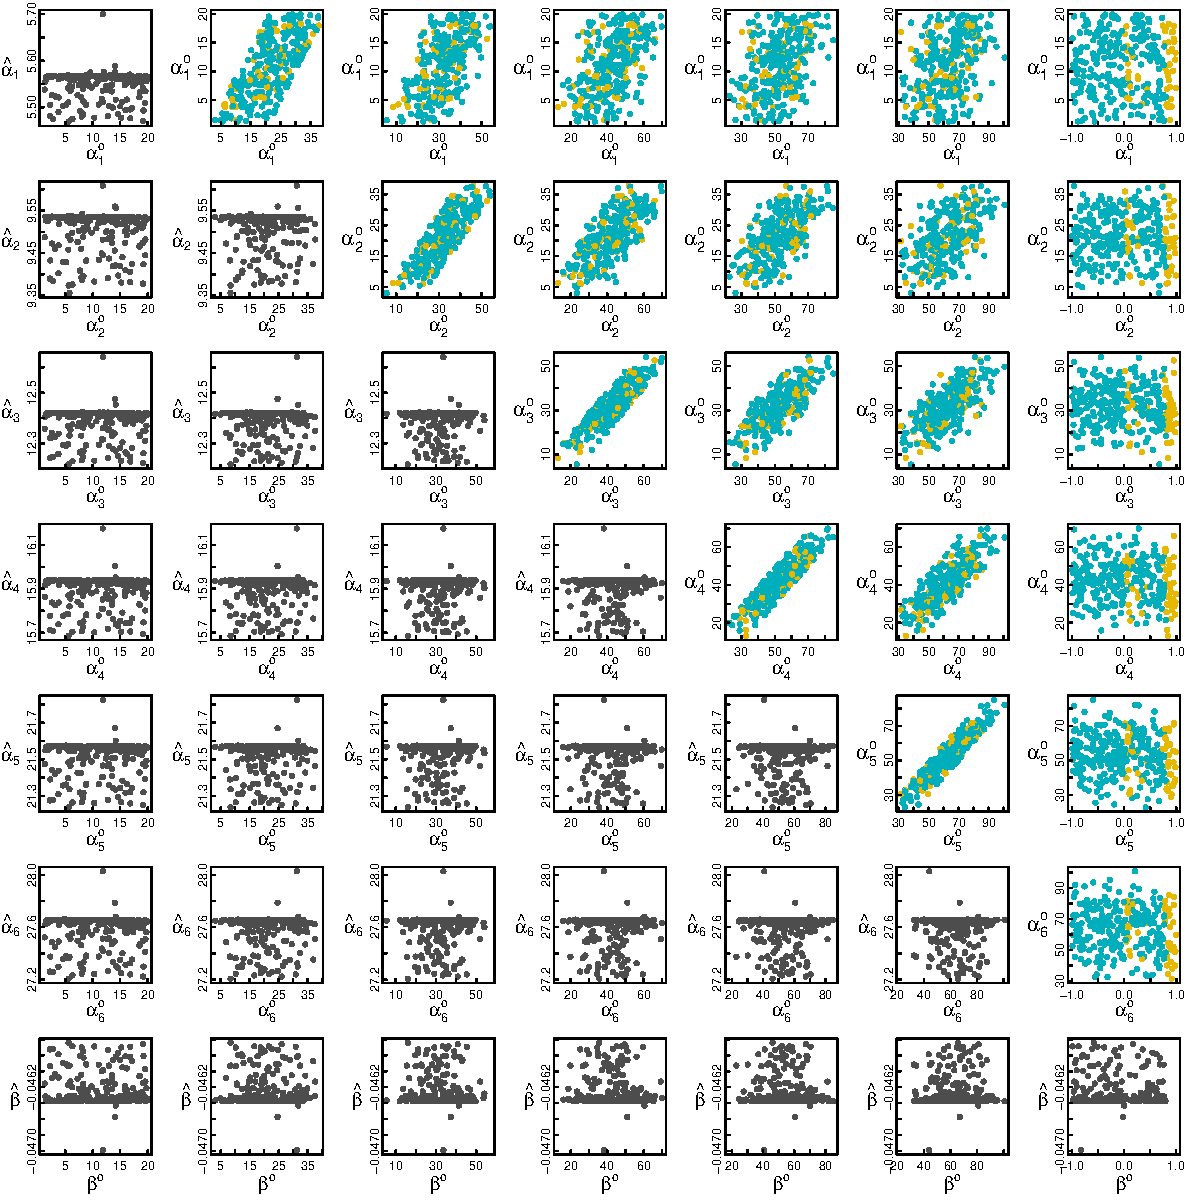
\includegraphics[width=\textwidth]{../figures/figS2_initial_value_sensitivity_logit.pdf}
  \caption{Sensitivity of optimisation results to initial values for the logit-link cumulative model with constant variance. The lower triangle and diagonal elements of the scatterplot matrix (grey symbols) show pairwise plots of filtered parameter estimates $\hat{\alpha}_i, \hat{\beta}$  against corresponding initial values $\alpha^{\circ}_i, \beta^{\circ}$. The upper triangle shows pairwise plots of the initial values for the same model parameters against each other. Green dots indicate successful convergence of the optimisation, yellow dots indicate convergence failures. Optimisation failed whenever $\beta^{\circ}>0.7$, furthermore convergence failures were more likely when $\beta^{\circ}\approx 0$.}
  \label{fig:figS2}
\end{figure} 

\begin{figure}[p]
  \centering
  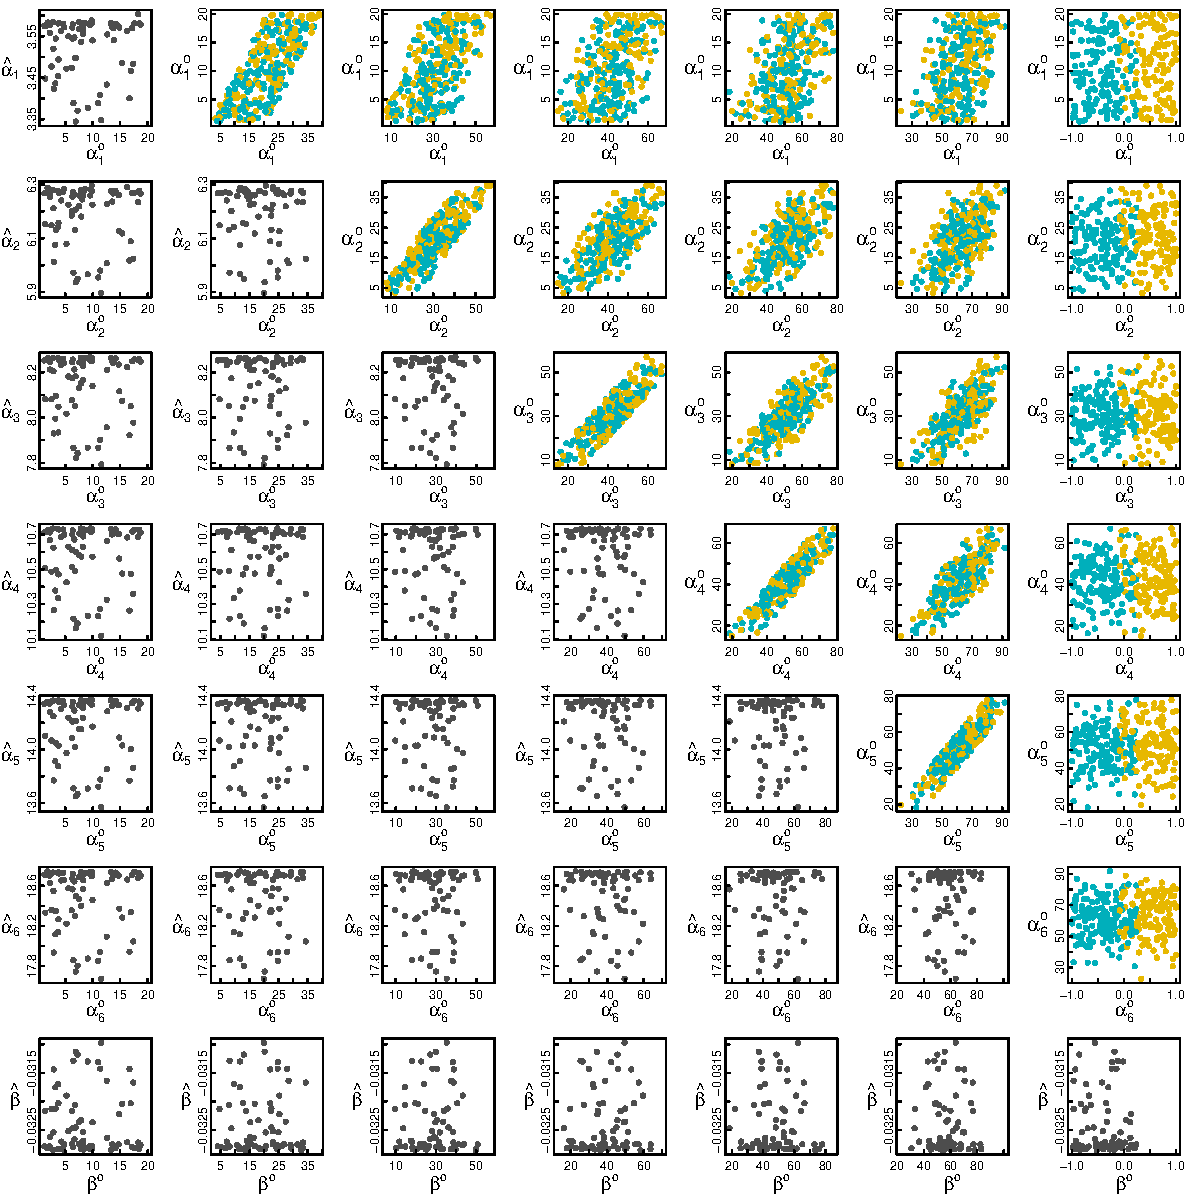
\includegraphics[width=\textwidth]{../figures/figS3_initial_value_sensitivity_cloglog.pdf}
  \caption{Sensitivity of optimisation results to initial values for the cloglog-link cumulative model with constant variance. The lower triangle and diagonal elements of the scatterplot matrix (grey symbols) show pairwise plots of filtered parameter estimates $\hat{\alpha}_i, \hat{\beta}$ against corresponding initial values $\alpha^{\circ}_i, \beta^{\circ}$. The upper triangle shows pairwise plots of the initial values for the same model parameters against each other. Green dots indicate successful convergence of the optimisation, yellow dots indicate convergence failures. Optimisation failed for most $\beta^{\circ}>0$.}
  \label{fig:figS3}
\end{figure} 